\section{Validation of the Estimator and of the Intervals}
\label{sec:validation}
\label{sec:validation_estimator}
\emph{In short: toy-MC experiments show an unbiased estimator at the minimum variance bound, intervals with nominal coverage and a test of $A=0$ with the nominal size.}
Toy-MC experiments generated from the fitted model of Sec.~\ref{sec:model} (Poisson yields, masses drawn from the model by the transformation method; $1000$ at the fitted value $A_{\mathrm{true}}=-0.0441$ and $300$ at each of $-0.1$, $-0.02$, $0$ and $+0.05$, each fitted with the nominal procedure, $1$--$3\%$ of the fits not valid and excluded) verify the estimator and the profile-likelihood ratio. Over the five values the bias of $\hat A$ is at most $0.0008$ ($1.6$ standard errors; $-0.0005$, $-0.0001$, $-0.0008$, $+0.0002$, $-0.0004$ for the five values; Fig.~\ref{fig:validation_injection}a), its spread equals the mean Hesse uncertainty within $6\%$ and the pulls have width $0.94$--$1.05$ (Fig.~\ref{fig:validation_injection}b): the estimator is \textbf{unbiased} and reaches the \textbf{minimum variance bound}.
At the fitted value the coverage of $t(A_{\mathrm{true}})\leq1$ is $0.696\pm0.015$ ($68.3\%$ level) and $0.954\pm0.007$ ($95.4\%$ level); the $68\%$ coverage over the five values is $0.71$, $0.70$, $0.69$, $0.69$ and $0.61$. %, the last, at $+0.05$ ($0.614\pm0.028$), $2.5$ standard deviations low, not unexpected among five values.
Inverting the Neyman construction, with $300$ toy-MC experiments at each of $11$ values of $A_{\mathrm{true}}$ between $-0.1$ and $0$, at the observed $\hat A$ gives the $68\%$ interval $[-0.0528,-0.0351]$, against the Minos interval $[-0.0526,-0.0356]$. The test of $A=0$ has the nominal size, $0.051\pm0.013$ at $A_{\mathrm{true}}=0$ against $0.05$, and $q(0)$ is compatible with $\chi^2_1$; Figure~\ref{fig:validation_injection} shows (a) the bias, (b) the spread and the pull width and (c) the size and the power of the test as a function of the injected asymmetry.

\begin{figure*}[!t]
\centering
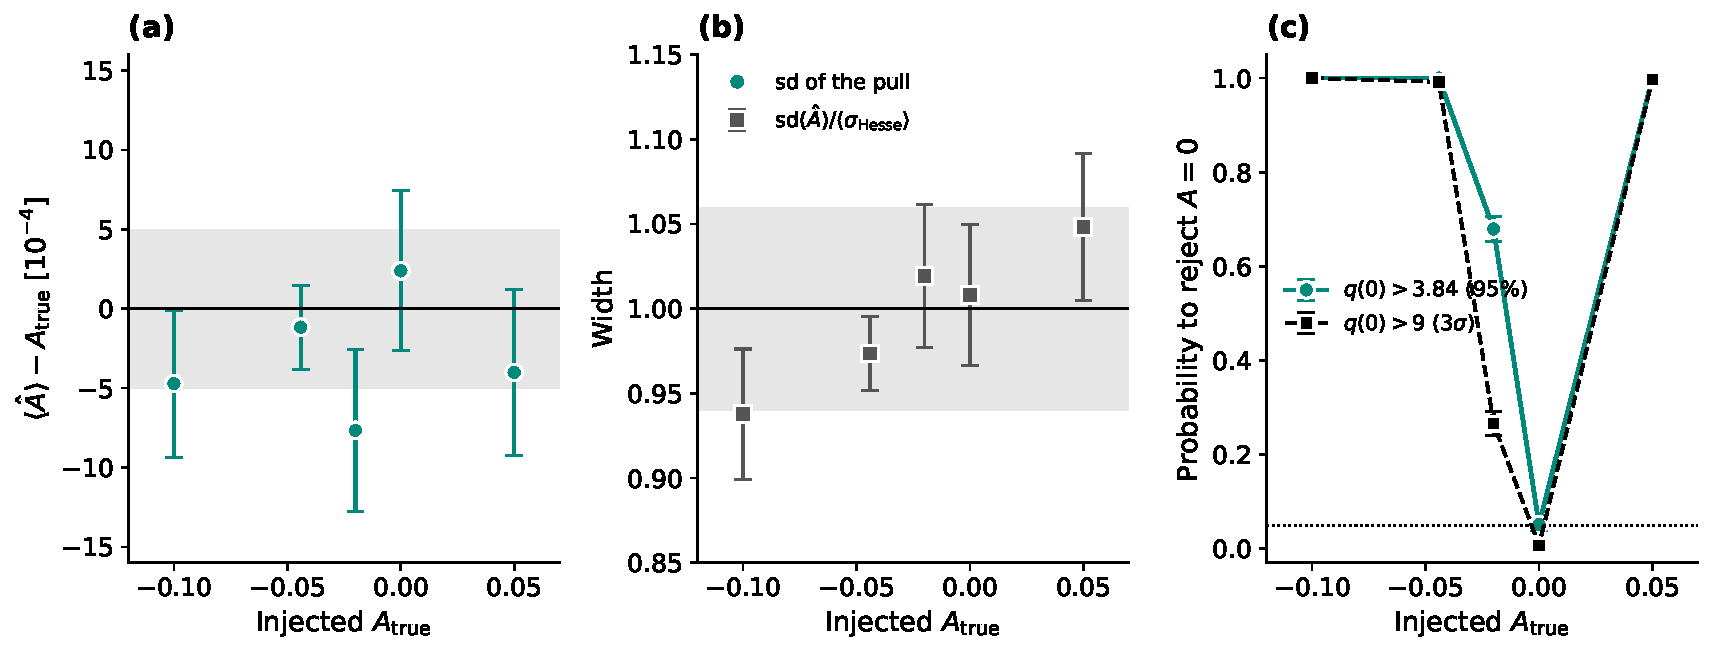
\includegraphics[width=0.95\textwidth]{figures/short_injection_power.pdf}
\caption{Toy-MC experiments at five injected asymmetries. (a) Bias of $\hat A$, with its standard error. (b) Spread of the estimates divided by the mean Hesse uncertainty, and width of the pulls. (c) Probability to reject $A=0$ in the test with $q(0)>3.84$ (size $5\%$) and $q(0)>9$ ($3\sigma$), as a function of the injected value: size at $A_{\mathrm{true}}=0$, power elsewhere.}
\label{fig:validation_injection}
\end{figure*}

%Under $A_{\mathrm{true}}=0$ the test $q(0)>3.84$ rejects in $0.051\pm0.013$ of the experiments, the \textbf{nominal size}, with $q(0)$ compatible with $\chi^2_1$ (Kolmogorov-Smirnov $p=0.79$); its power is $1.00$ at the fitted value and $0.68$ ($0.27$ at $3\sigma$) at $A_{\mathrm{true}}=-0.02$, so with $19{,}731$ candidates an asymmetry below $\sim0.02$ is \emph{not} resolved (Fig.~\ref{fig:validation_injection}c). The $5.2\sigma$ of the data is an extrapolation of the $\chi^2_1$ tail, which the $293$ experiments check only down to the $3\sigma$ level.

\subsection{Additional Results}
\emph{Asymptotic behavior.} With the number of candidates the bias tends to zero, the spread scales as $N^{-1/2}$ and the distribution of $\hat A$ becomes Gaussian.
\emph{Goodness of fit and binning.} The binned $\chi^2$ of toy experiments follows its asymptotic distribution, so its $p$-values are accurate: the misfit of the data is $5.4$ standard deviations in $10\,\MeV$ bins and $2.0$ in $2.5\,\MeV$ bins, because it lives on the scale of the flanks of the peak.
